\begin{frame}[fragile, t]{Figure environment}
    \begin{columns}[t]
        \begin{column}{0.5\textwidth}
        \begin{minted}{tex}
        In Figuur \ref{fig:squirrel} zie 
        je een eekhoorn:
        \begin{figure}[h]
            \centering
            \includegraphics[height=2cm]
            {squirrel.jpeg}
            \caption{Het beste dier. 
            Foto door Felix Rehm}
            \label{fig:squirrel}
        \end{figure}
        \end{minted}
        \vfill
        \end{column}

        \begin{column}{0.4\textwidth}
            \cmfontblock{
            \vspace{0.1cm}

            In Figuur \ref{fig:squirrel} zie je een eekhoorn:
            \begin{figure}[h]
                \centering
                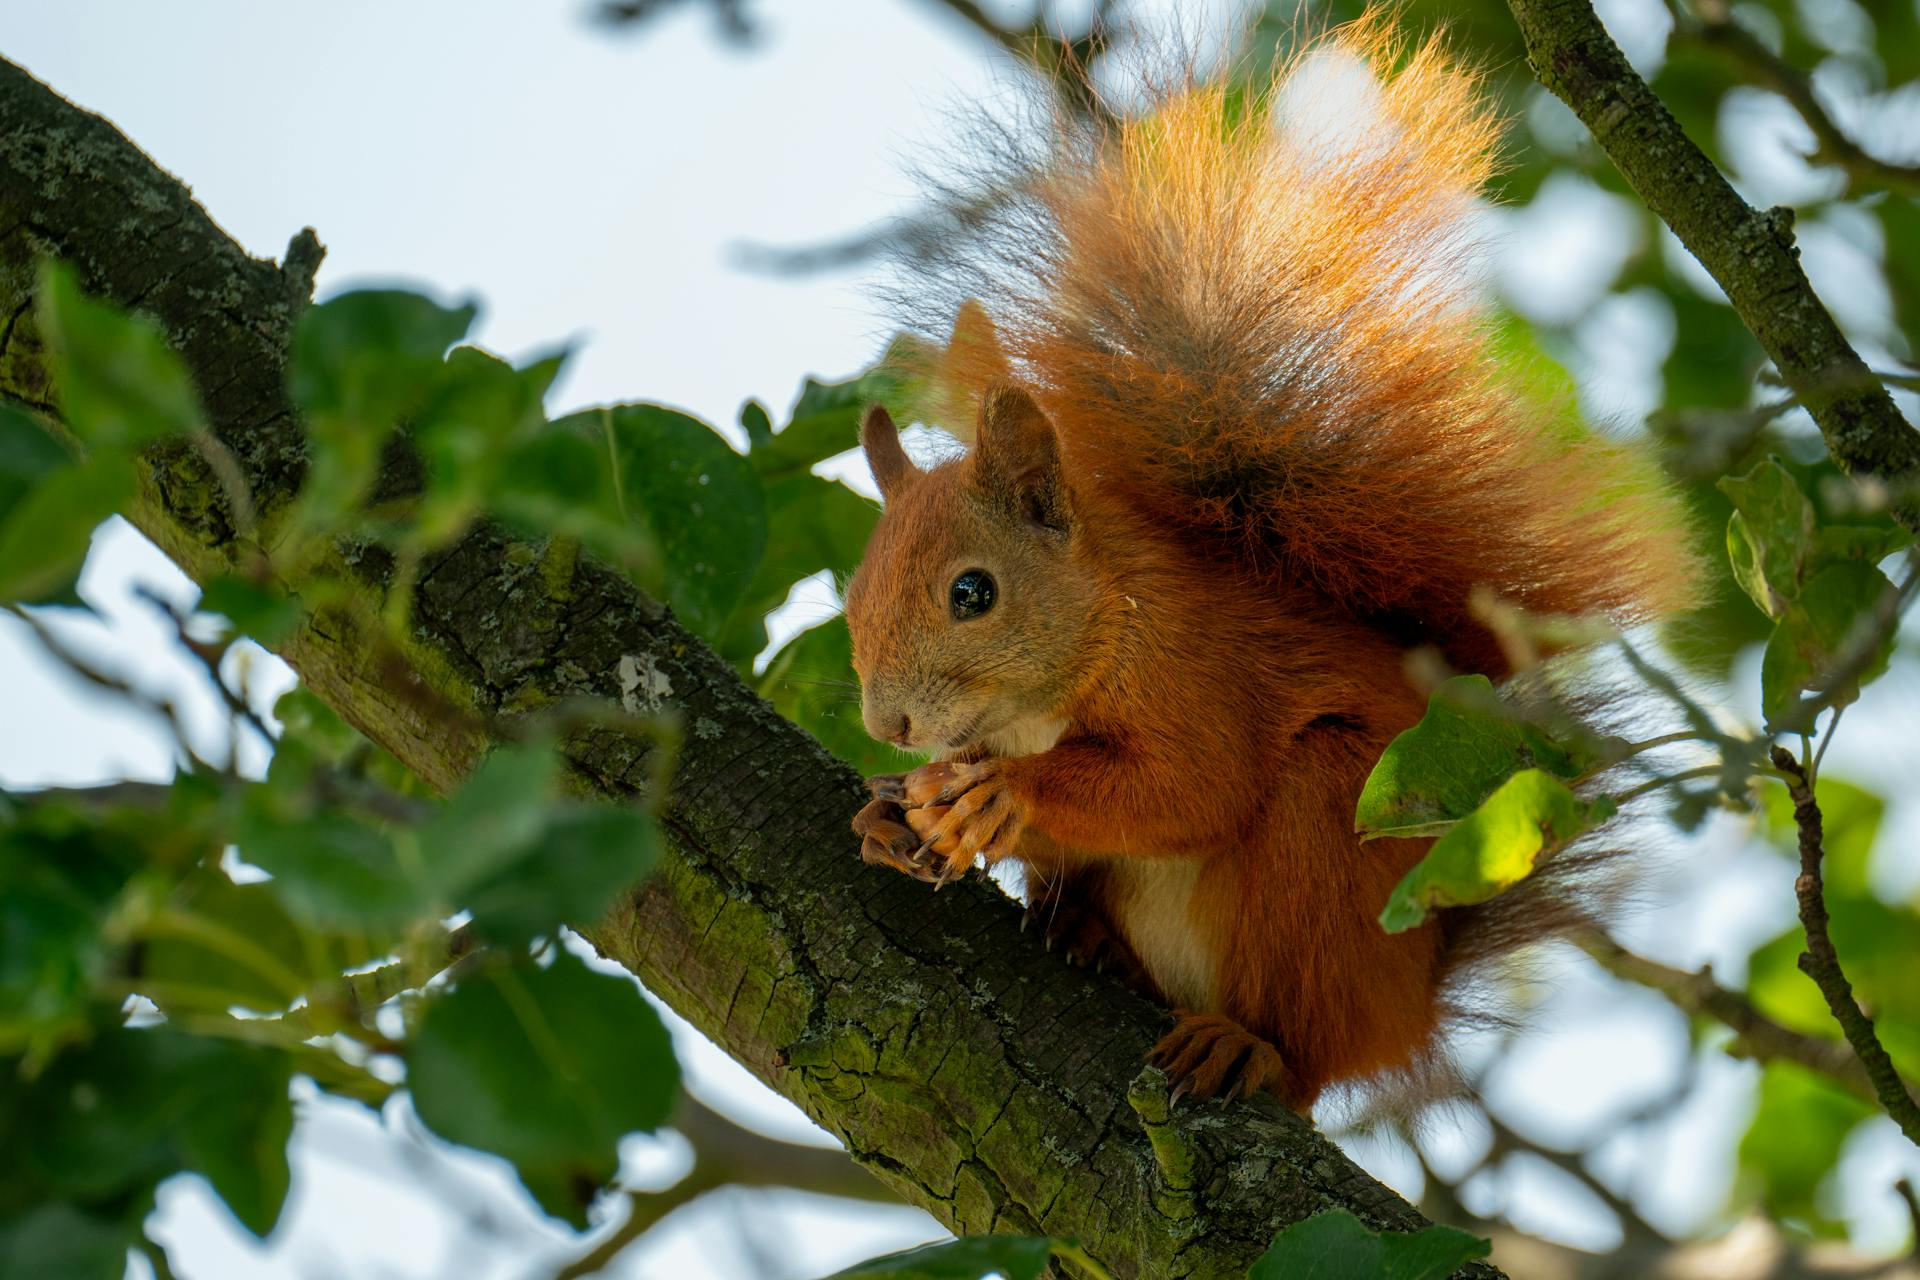
\includegraphics[height=2cm]{images/Foto_eekhoorn_FelixRehm.JPG}
                \caption{Het beste dier. 
                Foto door Felix Rehm}
                \label{fig:squirrel}
            \end{figure}
            }
        \end{column}
    \end{columns}
\end{frame}